\chapter{Reporting}\label{sec:Reporting}
Reporting is a core concept of Varroa.
Its purpose is to determine the results of a Varroa test and output them in a document.
The report is output as a PDF file and printed to the Commander's console.
For the latter an example is given in figure \ref{lst:ReportingOutput}.
\\
\begin{lstlisting}[caption={Excerpt from a reporting output}, captionpos=b, label={lst:ReportingOutput}, language=]
-------------- Commands  Report --------------
LifeCycle{lifeCycleId=s1.l1, clientGroupId=cg1, clientCount=100}
Connect{brokerAddress=broker.hivemq.com:1883}={
	durationSampler=[count=100, mean=228ms, stdDev=182ms, min=61ms, max=754ms],
	latenessSampler=[count=65, mean=210ms, stdDev=179ms, min=629us, max=654ms],
	failedCount=0}
Publish{pattern=topic/subtopic-[0-9], qos=1, count=1000, waitForAck=false}={
	durationSampler=[count=100, mean=10s, stdDev=7ms, min=10s, max=10s],
	latenessSampler=[-],
	failedCount=0}
Disconnect={
	durationSampler=[count=100, mean=4ms, stdDev=7ms, min=272us, max=27ms],
	latenessSampler=[count=12, mean=12ms, stdDev=4ms, min=3ms, max=17ms],
	failedCount=0}
---------------- End  Report -----------------
\end{lstlisting}
The results of a Varroa test are recorded per Action execution by a MQTT Agent.
The same Actions of different clients in the same Client Group are aggregated as a Action Report.
The list of all Action Reports forms the so called \emph{Actions Report} (see \ref{sec:actionsReport}).

Action Reports belonging to the same Command are further aggregated as a Command Report.
The list of all Command Reports compose the so called \emph{Commands Report} (see \ref{sec:commandsReport}).

For each of these Reports multiple metrics are output (see \ref{sec:metrics}).

\section{Commands Report}
\label{sec:commandsReport}
The Commands Report contains aggregated metrics for every Command.
They are output in the order in which the Commands were defined in the Scenario.
With the exception of nested Commands, where the metrics of the inner Commands are output before those of the outer Command.
An example is given in figure \ref{lst:CommandReport}.

\begin{lstlisting}[caption={Example for a Commands Report}, captionpos=b, label={lst:CommandReport}, language=]
-------------- Commands  Report --------------
Publish{[...]}
For{times=5}={[...]}
---------------- End  Report -----------------
\end{lstlisting}

\section{Actions Report}\label{sec:actionsReport}
The Actions Report allows for a more precise analysis of the Scenario than the Commands Report.
This is due to the fact that the Actions Report does not aggregate the metrics of nested Commands like the For Command.
Instead it outputs all iterations contained in the For Command separately.
This difference becomes clear when comparing figure \ref{lst:CommandReport} and \ref{lst:ActionReport}.
\begin{lstlisting}[caption={Excerpt from Actions Report}, captionpos=b, label={lst:ActionReport}, language=]
-------------- Actions  Report ---------------
Publish{[...]}
Publish{[...]}
Publish{[...]}
Publish{[...]}
Publish{[...]}
For{times=5}={[...]}
---------------- End  Report -----------------
\end{lstlisting}

\newpage
\section{Reporting Architecture}\label{sec:ReportingArchitecture}
\begin{figure}[H]
	\begin{center}
		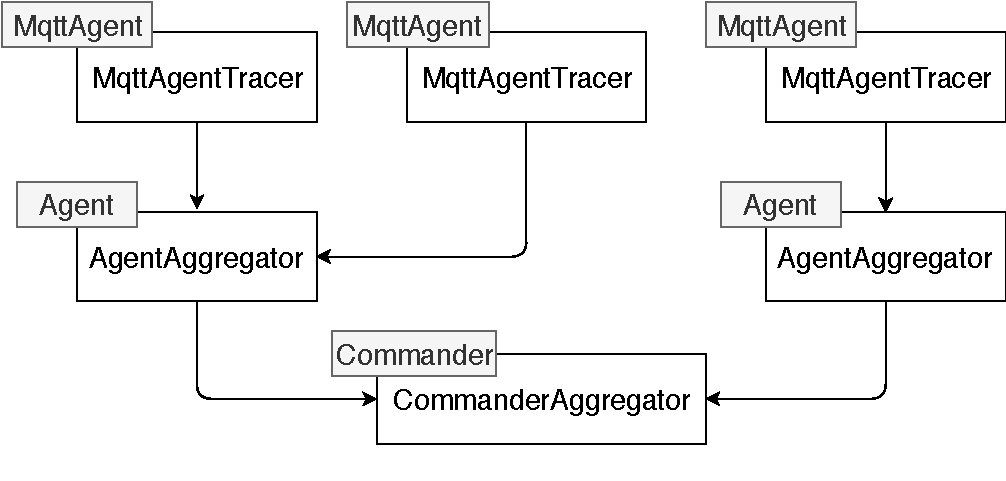
\includegraphics[scale=0.75]{Resources/PDF/ReportingArchitecture}
		\caption{Reporting Architecture}
		\label{fig:ReportingArchitecture}
	\end{center}
\end{figure}
The reporting architecture is organized in strong accordance to Varroa's hierarchy.
The data flow of the Action Reports happens bottom up from the Agents to the Commander.
The reported data is recorded at the lowest level of the hierarchy, the \emph{MqttAgentTracer} which tracks the MQTT Agent's Actions it belongs to.
Subsequently the \emph{AgentAggregator} receives this data and aggregates it before passing the result to the Commander.
The \emph{CommanderAggregator} collects the received data and then aggregates the information of all Agents and compiles it into the report.
Figure \ref{fig:ReportingArchitecture} visualizes the relationships between the components explained above.

\section{Metrics}\label{sec:metrics}
\subsection{Duration Sampler}
For every Action its duration is recorded.
The duration sampler aggregates these durations.
The following metrics are part of the duration sampler.
\begin{itemize}
	\item \textbf{count:} the amount of executed Actions.
	\item \textbf{mean:} the mean duration of the executed Actions.
	\item \textbf{stdDev:} the standard deviation of the duration of the executed Actions.
	\item \textbf{min:} the duration of the shortest Action execution.
	\item \textbf{max:} the duration of the longest Action execution.
\end{itemize}
\subsection{Lateness Sampler}
It is possible to specify an expected duration for each Command.
The actions exceeding this limit get recorded by the lateness sampler.
The following metrics are based on the delta of the expected duration and the actual duration.
\begin{itemize}
	\item \textbf{count:} the amount of Actions whose durations exceeded the expected duration.
	\item \textbf{mean:} the mean lateness delta.
	\item \textbf{stdDev:} the standard deviation of the lateness delta.
	\item \textbf{min:} the minimum lateness of the executed Actions.
	\item \textbf{max:} the maximum lateness of the executed Actions.
\end{itemize}

\subsection{Failed Count}
Another important metric is the count of failed Actions.
It indicates how many of the Actions could not be executed successfully.



